%PART_3_CHAP_3_SEC_3
%WAIT a Review, ok
\clearpage
\section{Motivation}\label{chap:3.2}
    \subsection{Introduction}
        Pour cette thématique de la motivation, trois expérimentations sont ici présentées. La 1\iere est une proto-étude qui n'a jamais donné lieu à des passations expérimentales à proprement parler, mais qui a fourni plusieurs pistes de recherche et prétexté la construction de plusieurs ressources méritant d'être mentionnées. L'expérimentation suivante met en jeu le robot Poppy Dragster et sa notice de montage: ce robot développé dans l'optique de constituer une activité en soi pour le robot Ergojr, comme dérivation de celui-ci, donne une autre dimension à sa notice de montage qui devient alors une ressource pédagogique à part entière. Deux versions de cette notice ont été produites et sont ici comparées, notamment en terme d'efficacité dans la réalisation de la tâche mais aussi sur la perception par l'élève de la controlabilité de la tâche grâce au questionnaire \sht{IMI}. Enfin, la 3\ieme expérience propose d'étudier l'impact de la formulation des ressources pédagogiques sur, d'une part, la difficulté perçue (également via le \sht{IMI}) et, d'autre part, sur la compréhension des notions abordées dans l'activité. Mais, cette seconde sera abordée en section suivante~\citeS{chap:3.3}.
    \subsection{Proto-expérience}
        %\paragraph{\textit{Exp}: \cro{les a-priorie en robotique}}\label{Exp:a_priorie}
            %Il s'agit d'évaluer ici l'envie et la difficulté perçue par l'apprenant à réaliser une activité robotique. Deux contexte: les élèves entrent dans la salle de \sht{TD} où le matériel est pré-positionné; \Li présenter l'activité dans le détail et répondre à toutes les questions qui seront posées, ou \ii ne rien faire. Puis demander à l'apprenant d'estimer la difficulté de la tâche en fonction de ses capacités~\citeB{bandura1986explanatory} \ie \cro{vous vous sentez capable d'accomplir cette tâche} oui/non; puis d'estimer le degré de certitude de sa réponse (via une échelle likert) et de même sur son envie~\citeB{atkinson1957motivational}. Faire réaliser l'activité. Enfin, demander s'il pense avoir réussi l'activité et pourquoi~\citeB{weiner1985attributional}. Ce type de protocole peut être intégrater avec de multiple types de d'activité. 
        \paragraph{\textit{Exp}: \cro{Rôle du support}}\label{Exp:Role_support}
            Ici, l'objectif de ce protocole est de mettre en évidence les difficultés de gestion des différents supports durant l'activité et les effets de double tâche induits par cela~\citeS{sec:double-tache}.
            Ici, la même activité (\eg thème, question posée, information donnée, \etc) est proposée au sujet selon quatre formats: \Li un support \sht{pdf} présenté numériquement, \ii présenté en version papier, \iii adapté en vidéo et \iiii intégré directement dans l'interface de programmation (dans notre contexte \sht{snap}). L'hypothèse serait que le \Li n'offrirait aucun avantage face à sa version papier, comme ce que nous avons constaté~\citeS{sec:support}. En revanche, les difficultés d'utilisation d'un même écran \tiret{alternant interface de programmation et ressources vidéos} ne garantissent pas son avantage sur les ressources papiers. De même, le format intégré, et la perte de contrôle qu'il implique~\citeS{sec:contro} ne garantissent pas son avantage sur un format vidéo ou même papier.
            \subparagraph{Matériels vidéo}
                À ces fins, 3 vidéos ont été réalisées~\citeURL{TD-chicken-td} et les premières ébauches de l'activité \cro{poule}~\citeS{sec:act_poule} et de la démo \cro{têtu} ont été créées.
                La vidéo1 présente l'environnement \sht{snap}: comment créer une variable et la modifier. Elle montre ensuite comment accéder à une catégorie et déplacer un bloc. Ainsi, 2 blocs sont alors posés sur la zone de script: 'set position' et 'all motors' permettant respectivement de déplacer un moteur dans une position; et de récupérer le nom des moteurs du robot. Puis elle réutilise la variable créée ultérieurement, en l'insérant dans le bloc \cro{set position}, elle correspond ainsi à la valeur en degrés de la position à atteindre. Enfin, elle montre comment attribuer une variable à chacun des 3 moteurs de la base du robot et introduit le bloc 'forever' (pour toujours); ce petit code permet ainsi de déplacer le robot réel et virtuel grâce à la manipulation des variables. Quatre notions sont ici développées: créer/modifier une variable; répartition des blocs en catégories; contrôler le robot; la boucle 'forever'
                Ils sont alors invités à réaliser eux-mêmes ce qu'ils viennent de voir et à faire leurs propres tests. C'est à ce moment qu'ils commencent à coder et manipuler le robot. Quinze minutes après le début de l'activité ils sont invités à regarder la deuxième vidéo.\par%
                La vidéo2 présente un algorithme à réaliser: le \cro{comportement poule}. L'objectif est de contrôler les 3 moteurs supérieurs (m4, m5, m6) via les 3 moteurs de la base (m1, m2, m3), pour qu'ils compensent leurs mouvements (exemple: si m1=+30° alors m4=-30°). La première étape présente comment simplifier (optimiser/factoriser) les écritures en utilisant les listes. Puis, est montré comment associer les moteurs entre eux (assemblage de plusieurs blocs). Enfin comment (via le bloc 'map') inverser la valeur des positions des moteurs de la base. Pour terminer, une démonstration de l'exécution du programme sur le robot réel et sur le robot virtuel est fournie. Trois notions sont ici développées: créer/modifier une liste; récupérer les informations des senseurs du robot; consolider les manipulations précédentes.\par%
                30 min plus tard, la vidéo3 propose un défi: réaliser le \cro{comportement têtu}. Elle commence par une démonstration du comportement sur le robot réel. Puis elle fournit l'algorithme qui produit ce comportement: \gui{je me souviens de ma position de départ. Pour toujours, si j'ai bougé: alors, je retourne dans ma position de départ, sinon, j'attends 1 seconde.} Un certain nombre d'indices/astuces sont fournis jusqu'à la fin de la vidéo pour réussir à coder ce comportement en moins de 45min.
            \subparagraph{Limite}    
                Cependant, la difficulté de produire des vidéos évoluant aussi rapidement que le matériel \sht{pdf} nous a empêché de mener à bien ce type d'expérience. De plus, il en est de même pour les supports intégrés qui \tiret{pour permettre une ergonomie de mise à jour suffisante} auraient nécessité un investissement trop grand. En revanche, un didacticiel directement intégré à \sht{snap} a été réalisé dans ce sens, mais n'a pas donné suite. Il est aujourd'hui toujours disponible en ligne~\citeURL{TD-discover-td}, il se compose d'une phase interactive de découverte (environ 45min) puis d'une phase pratique de programmation où l'utilisateur applique les notions abordées précédemment, puis après un temps défini (45 min par défaut), une série de comportement est présentée et explicitée pendant environ 30min (phase passive). Dans sa forme actuelle, ce didacticiel est trop \cro{riche} d'informations pour permettre leur bonne assimilation; cependant, il offre un bon complément pour des personnes averties. 
    %dragster
    \subsection{\textit{Exp}: \cro{Notice modulaire ou linéaire} }\label{Exp:dragster}
        \myPhantom{paragraph}{Introduction}
            Nous voulons évaluer ici la perception de la contrôlabilité~\citeS{sec:viau} des étudiants et voir l’impact des différentes pratiques d’activités sur leur apprentissage, leur satisfaction et leur perception des tâches.
            La perception de la contrôlabilité correspond au niveau de contrôle que les étudiants pensent avoir sur la réalisation de l'activité et de ses résultats. Cela peut être créé en responsabilisant les étudiants, en les laissant faire des choix. Nous voulons donc avoir un groupe qui fera des choix entre plusieurs options proposées, tandis que l’autre groupe devra suivre les instructions pas à pas.
            L’autorité et le monopole du professeur peuvent faire tomber ce sentiment de choix, c’est pourquoi nous devrions intervenir le moins possible avec le groupe sauf si cela est nécessaire, ne pas leur donner des instructions autoritaires et les laisser prendre leurs décisions jusqu’à ce qu’ils nous appellent pour validation. Notre objectif est de concevoir des activités d’assemblage pouvant être présentées sous un format linéaire (instructions à suivre pas à pas) ou sous un format modulaire (différentes feuilles à choisir).
        \paragraph{Méthode}
            Étant donné que c’est la première fois que le robot Dragster est présenté et utilisé par les étudiants, nous souhaitons mettre l’accent sur l’assemblage plutôt que sur les activités de programmation. Les activités de programmation seront les mêmes pour les deux groupes, l’assemblage sera différent. C'est pourquoi les étudiants seront répartis en deux groupes, chaque groupe se trouvant dans une pièce différente.
            \subparagraph{Population}
                Les sujets venaient visiter le centre Inria Sud-Ouest, ils étaient donc disponibles le matin pour l'expérience. Comme ils avaient tous moins de 18 ans ($\overline{x}=$16~ans), un formulaire de consentement signé par les parents était obligatoire~\citeS{sec:adm}.
                Il y avait 35 étudiants: 12 filles et 18 garçons, de 1\iere S3 lycée La Sauque, ils ont été divisés en 2 groupes: \sbg{GM}, 15 étudiants (5 groupes de 3); \sbg{GL}, 15 étudiants (5 groupes de 3); 5 autres étaient dans un groupe qui n'a pas participé à l'étude.
            \subparagraph{Hypothèses}
                Selon le modèle Viau de motivation de l'étudiant, les étudiants peuvent influencer positivement leurs progrès sur l'activité par leurs choix, en se sentant responsables et en contrôle. Ainsi, le groupe avec l'assemblage présenté dans un format modulaire (GM) devrait se sentir plus en contrôle avec un sentiment de choix plus élevé et avoir plus de progrès dans l'activité d'assemblage.
                Ainsi, nos hypothèses sont que le groupe \sht{GM} sera plus satisfait (plus de plaisir et plus de choix) et plus efficace (moins d'effort et plus rapide) en ce qui concerne la réalisation de la tâche en raison de la liberté de choix induite par les différents modules.
            \subparagraph{Matériel}
                Guide de montage et de configuration \sht{GL}~\citeA{pdf:notice_dragster_lin}, le tout dans une feuille continue. La fiche d'activité est remise aux étudiants avec les pages jointes. Ils suivent donc les tâches une à une (assemblage électronique, configuration du moteur, assemblage mécanique de la base puis du bras, test du robot) selon l'ordre imposé.
                Guide de montage et de configuration \sht{GL}~\citeA{pdf:notice_dragster_mod}, séparé en 8 feuilles différentes. Les instructions sont écrites sous la forme passive pour donner la liberté dans les actions au lieu de donner des instructions (par exemple: \cro{les moteurs peuvent être configurés en entrant cette commande} au lieu de \cro{définir les moteurs avec cette commande}). Les étudiants peuvent choisir la feuille de départ même s'il y a des actions à faire avant d'autres (le test ne peut pas être effectué si les moteurs ne sont pas configurés). Si ce cas arrive, les étudiants doivent se rendre compte qu'ils doivent effectuer des tâches préliminaires.\\
                \begin{figure}[!h]
                    \centering\label{fig:drag_proto}
                    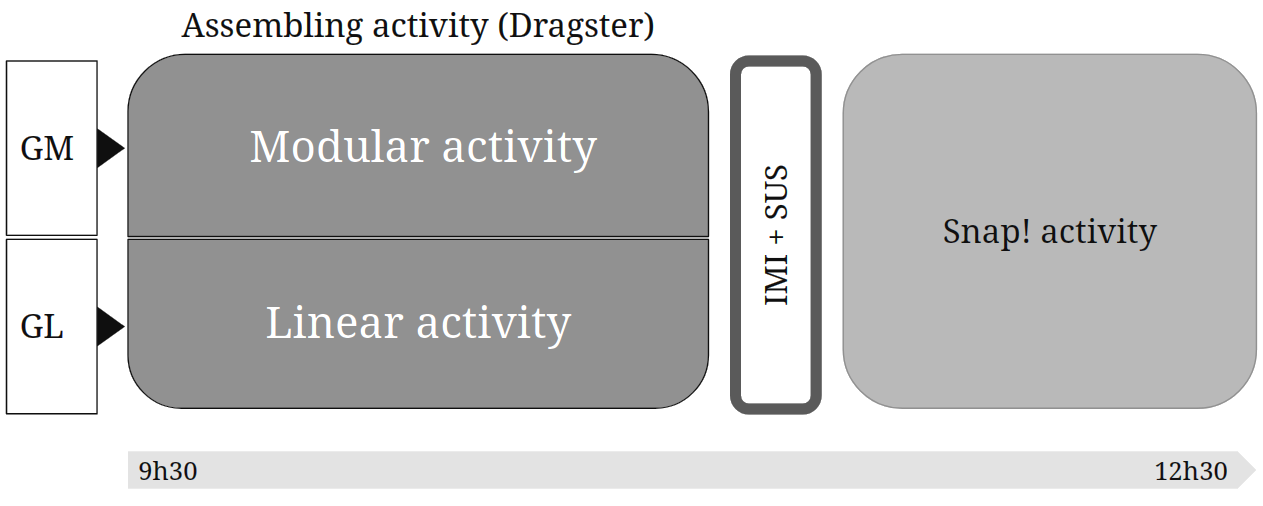
\includegraphics[width=0.9\linewidth]{Figures/Gilliard-proto.png}
                    \caption{Protocole: \cro{Notice modulaire ou linéaire}}
                \end{figure}
                Une même activité a été proposée après le montage du robot~\citeA{pdf:act_dragster}. Elle permettait, entre autres, de remarquer et de corriger les erreurs potentielles lors du montage. L'activité explorait les fonctions de base telles que le déplacement d'un moteur, puis un peu plus complexes avec de la détection d'objets basée sur la boucle sensori-motrice.\par%
                Entre le montage et l'activité, deux questionnaires individuels ont été complétés par les étudiants: le \sht{SUS}~\citeS{q:sus} et 4 sous-échelles du \sht{IMI}: Intérêt~/~plaisir, Compétence perçue, Effort~/~Importance, Choix perçu~\citeS{q:imi}. Les réponses recueillies sur papier ont été extraites avec \sht{amc}. Un test de Student unilatéral pour deux échantillons à variance inégale est utilisé pour estimer la significativité des résultats.\par%
                L'expérimentation (accueil et répartition des groupes / montage du dragster / questionnaires / activités) se déroula sur une matinée entière: de 9h30 à 12h30.
                Au préalable, une étude pilote sur 3 étudiants de 22 ans (qui n’avaient jamais programmé auparavant) a été réalisée afin de détecter les erreurs potentielles dans les fiches d’activités, les images ou informations manquantes et également de vérifier l'estimation du temps de construction du dragster. Les résultats et les retours d'expérience de l'étude pilote nous ont aidés à clarifier des parties importantes et à confirmer la validité des activités.
        \paragraph{Résultats}
            Suite à l'expérimentation, nous observons~\citeF{fig:result_dragster} que, concernant l’assemblage, il existe une différence significative (test de Student, $p=1.88e-10$) entre \sht{GM} ($\overline{x}=62$ minutes). et \sht{GL} ($\overline{x}=109$ minutes). Pour le test \sht{IMI}, les résultats montrent qu'il existe une différence significative positive pour \sht{GL} avec l'échelle \cro{choix} ($p=0,04287$). Nous  notons, qu'il n’y a aucune différence entre les groupes pour les autres échelles \sht{IMI} \cro{compétence} ($p=0,37849$), \cro{plaisir} ($p=0,39675$) et \cro{effort} ($p=0,21155$); ni pour le SUS ($p=0.24412$).
            \begin{figure}[!h]
                \centering
                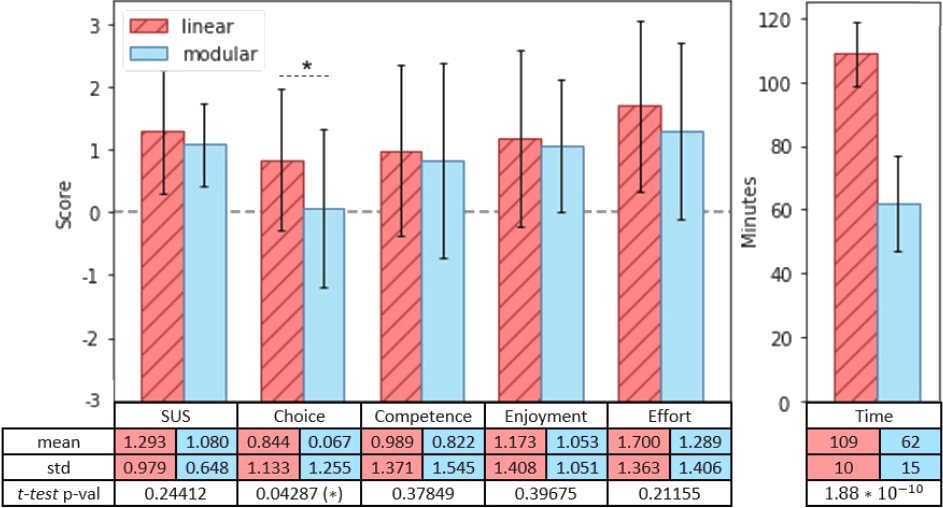
\includegraphics[width=0.9\linewidth]{Figures/Gilliard-result}
                \caption{Résultats, \cro{Notice modulaire ou linéaire}}
                \label{fig:result_dragster}
            \end{figure}
        \paragraph{Conclusion}
            %les résultats ont montré que la contrôlabilité et le choix dans une activité modulaire placeraient les étudiants dans une attitude plus \cro{active}, même s'ils ont le sentiment d'avoir eut moins de choix
            Le groupe \sht{GM} était presque deux fois plus rapide que le groupe \sht{GL}. Cela pourrait s'expliquer par le fait que la tâche d'assemblage était plus facile à répartir entre les trois membres de chaque groupe en raison des feuilles séparées (par exemple, on peut assembler des roues tout en assemblant des bras). Dans les observations, presque tous les groupes \sht{GM} se sont divisés en tâches tandis que dans le groupe \sht{GL} certains membres étaient totalement passifs. Ainsi, notre hypothèse sur le temps d'assemblage qui diffère entre les groupes est acceptée.
            sur les aspects motivationnels, nous nous attendions à un sentiment plus important de liberté de choix dans le groupe \sht{GM} en raison de la possibilité de choisir entre les feuilles et le vocabulaire utilisé (suggestions et non ordres). 
            Cependant, l’échelle \cro{Choix} est significative mais est à l’inverse de ce que nous avions prédit: le sentiment de choix est plus élevé pour le groupe \sht{GL}. Ainsi, notre hypothèse sur le sentiment de choix plus élevé pour le groupe \sht{GM} est rejetée. Ce résultat pourrait être dû au fait que les organisations internes de chaque groupe d'élèves fait émerger une forme de leadership qui pourrait induire une forme de contrainte au sein des groupes et réduire le sentiment de choix.
    %poule
    \subsection{\textit{Exp}: \cro{Décrire ou manipuler}}\label{Exp:poule}
        \myPhantom{paragraph}{Introduction}
            Nous voulons ici évaluer l’impact de la manipulation tangible~\citeS{sec:tangible}  sur les étudiants. Une manipulation tangible peut créer une immersion dans l'expérience. Il peut soutenir la cognition spatiale des utilisateurs, réduire la charge cognitive et permettre une immersion plus créative dans le problème. Cela peut également donner plus d'autonomie à l'apprenant, lui permettant de corriger ses erreurs et de comprendre les concepts abstraits qui se cachent derrière. Il est déjà apparu comme un support efficace pour la programmation. En plus d’avoir accès en classe à leur robot, nous souhaitons que les étudiants profitent des possibilités de manipulation: le robot n’est ni fragile, ni dangereux, ni simple à manipuler. Nous voulons les amener à être plus actifs dans la manipulation et à tester si cela affecte leur perception de l'activité et les résultats du quiz.
        \paragraph{Méthode}
            Nous avons décidé de créer deux situations d'apprentissage: l'une axée sur la démonstration (l'étudiant doit reproduire l'action présentée), l'autre sur la description (l'étudiant doit reproduire l'action décrite). Nous voulions une action simple impliquant des boucles sensori-motrices afin que les étudiants puissent manipuler leur robot avec leurs mains et avoir un retour direct. Un \cro{comportement animal} semblait adapté et intéressant à recréer.
            Pour ce faire, nous présentons à chaque groupe une activité de quatre pages~\citeA{pdf:act_poule}. Seule la dernière page diffère des autres en fonction de \cro{Description} ou \cro{Démonstration}~\citeF{fig:act_poule}. Ils doivent reproduire le mouvement d'une \cro{poule} (la tête du robot reste stable lorsque son corps est déplacé), soit en observant et en manipulant son robot, soit en suivant une liste de conseils pour créer le comportement souhaité. Avant de commencer la dernière page, une vidéo du comportement d'une poule~\citeURL{TD-chicken-move}  est affichée.
            \subparagraph{Population}
                Les sujets étaient des lycéens de lycées en partenariat avec Inria~\citeS{sec:etablisements}.
                Il y avait 66 étudiants du lycée St Genes et du lycée Condorcet. 14 élèves ont été retirés parce qu'ils n'avaient pas terminé l'activité évaluée ou n'avaient complété l'ensemble des pages des questionnaires; 24 étaient des filles, 28 des garçons, d'une moyenne d'âge de 15 ans. À chaque intervention, le groupe d'élève était divisé en deux groupes: \sht{GDemo} et \sht{GDesc}. Les 54 étudiants formaient un ensemble hétérogène: certains étaient issus de filière \cro{scientifique}, d'autres de filière \cro{littéraire} mais aucun n'avait effectué d'activité robotique en classe.
            \subparagraph{Matériel}
                L'activité proposée possédait deux variantes~\citeS{sec:act_poule}. En fin d'activité, chaque étudiant complétait un quiz composé de 6 questions portant sur les notions abordées dans l'activité~\citeA{pdf:qcm_poule}; puis il complétait 4 sous-échelles du \sht{IMI}: Intérêt~/~plaisir, Compétence perçue, Effort~/~Importance, Pression~/~tension~\citeS{q:imi}.
            \subparagraph{Hypothèse}
                La manipulation tangible peut conduire à une plus grande immersion dans le problème et peut donner plus d'autonomie à l'apprenant, permettant de corriger soi-même les erreurs et de comprendre les concepts plus précisément~\citeS{sec:tangible}. Pour nos hypothèses, nous nous attendons à ce que la manipulation tangible ait un impact plus fort sur les résultats d'apprentissage évalués par le quiz du groupe de démonstration. Les autres échelles du \sht{IMI} sont utilisées à titre exploratoire et pourraient nous aider à mieux interpréter les résultats.
            \subparagraph{Déroulement}
                Tous les étudiants arrivent en classe en même temps et sont assis par groupes de deux étudiants par table et avec un ordinateur et un kit robotique.
                Qu'ils soient dans le groupe \cro{Description} ou \cro{Démonstration}, ils font tous, les trois premières feuilles d'exercices à la vitesse qu'ils désirent. Nous leur donnons les feuilles une par une. Ils doivent donc nous appeler quand ils ont terminé avec une feuille pour obtenir la suivante. Avant de leur donner la feuille suivante, nous effectuons une rapide vérification avant qu’ils ne continuent. Comme les premières feuilles sont plus faciles que la quatrième, ils sont assez autonomes dans leur travail. Ils sont autorisés à parler avec leur partenaire, cependant, ils ne doivent pas communiquer avec d'autres groupes. 
                Finalement, quand ils ont fini avec la troisième feuille, ils commencent le \cro{défi poule} qui est la partie qui nous intéresse. Ils regardent la vidéo de démonstration et commencent à créer leurs fonctions avec \sht{snap}. 1h50 après leur entrée en classe, par contrainte de temps, ils doivent s'arrêter là où ils sont et remplir le quiz puis le questionnaire. Une fois qu'ils ont terminé, ils peuvent quitter la classe.
                Les réponses collectées sont extraites avec \sht{amc} et converties en fichiers csv. Un test de Student unilatéral pour deux échantillons à variance inégale est utilisé pour estimer la significativité des résultats.\par%
                Nous avons organisé 6 sessions de notre expérience, toutes entre mai et juin. Au préalable, nous avions effectué une étude pilote sur 5 lycéens (1 groupe de 3 et 1 groupe de 2) avec ErgoJr au centre Inria avant de faire des expériences en classe. Cela nous a permis d'ajuster et de clarifier certaines instructions. Nous avons également rencontré les enseignants et visité les deux salles de classe une semaine avant pour vérifier l’ordinateur, la connectivité et les détails techniques afin de s’assurer que tout fonctionne directement le jour des expériences.
        \paragraph{Résultats}
            Pour le groupe \sht{GDemo} la perception de la quantité d'effort à fournir pour réaliser l'activité est plus faible que pour le groupe \sht{GDesc} ($p=0.042$) et ils obtiennent un score plus élevé au quiz ($p=0,067$). Nous observons également que les échelles de compétence, d’effort, d’intérêt et de quiz sont positives pour les deux groupes, tandis que l’échelle de pression est négative. Cependant, les échelles Compétence, Intérêt et Pression ne sont pas significativement différentes entre ces deux groupes.
            Les résultats concernant le quiz sont détaillés dans la section suivante~\citeS{Exp:poule_2}
            \begin{figure}[!h]
                \centering
                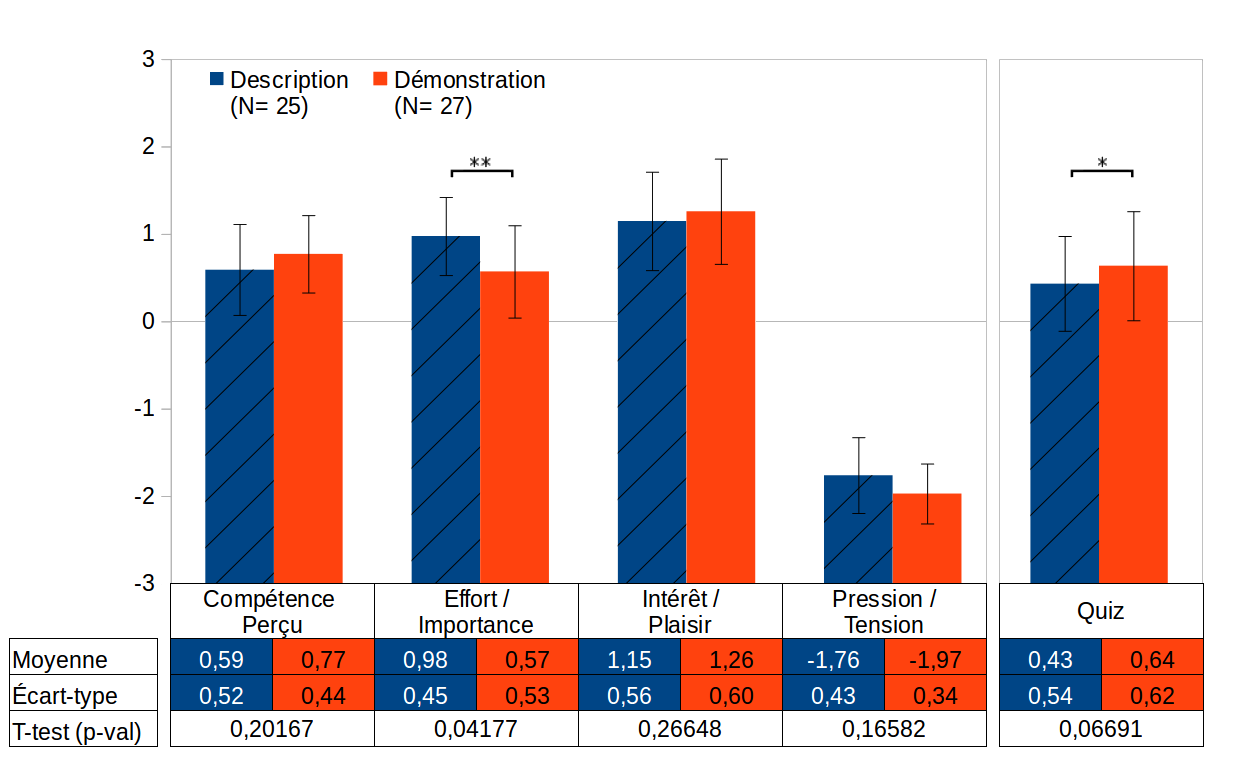
\includegraphics[width=0.9\linewidth]{Figures/Desprez-result_poule.png}
                \caption{Résultats globaux \cro{Décrire ou manipuler}}\label{fig:result_poule}
            \end{figure}
        \paragraph{Conclusion}  
            L’étude a été répliquée dans 6 contextes différents, à chaque fois, le groupe d'élèves fut réparti entre les deux conditions \sht{GDemo} et \sht{GDesc}. Même si les groupes sont hétérogènes, cela permet d’avoir une étude beaucoup plus réaliste et écologique qui s’adapte à la variabilité naturelle de notre population de \gui{lycéens} (variant entre deux lycées avec des étudiants de différents parcours, origines, motivations, \etc). Nous constatons qu'une activité mettant en jeu une démonstration tangible des objectifs à atteindre permet de réduire l'effort perçu par l'élève et potentiellement de lui offrir de meilleurs résultats en terme d'acquisition de connaissances.
    \subsection{Synthèse}
        Les expériences ici menées ne nous permettent pas d'observer si il existe un avantage à exercer une activité robotique (en matière de gain motivationnel) comparé à une activité lambda. Cependant, on note que \Li l'obligation de telles pratiques (via les programmes officiels) rend cette distinction peu pertinente (les deux types d'activités devant être réalisés pour d'autres raisons que le seul aspect motivationnel); et que \ii la proximité d'aujourd'hui entre technologie robotique et nouvelles technologies rend les résultats, qui seraient obtenus pour cette distinction, peu pérennes.
        Ainsi, nous avons choisi d'aborder les caractéristiques de mise en place des activités robotiques et leurs impacts motivationnels relevés ici via le questionnaire \sht{IMI}. Nous avons observé dans une première expérience que lors d'une tâche de construction d'un robot le sentiment de contrôle sur l'activité variait avec le format des ressources fournies (\eg modulaire \textit{vs} linéaire): l'activité modulaire, bien que, objectivement plus libre dans sa réalisation, a obtenu le sentiment de contrôle le plus faible. Dans une seconde, nous avons vu que dans le cadre d'un \sht{TD}, la formulation et les démonstrations fournies impactaient le sentiment d'effort: une démonstration tangible semble permettre une meilleure compréhension de l'objectif à atteindre et donc de l'effort à fournir pour sa réalisation; pour s'en assurer, il faut mesurer si les élèves ont objectivement mieux compris les concepts nécessaires à la réalisation de l'objectif. 